\documentclass[11pt,a4paper]{article}

\usepackage[T1]{fontenc}
\usepackage[utf8]{inputenc}
\usepackage[frenchb]{babel}

\usepackage{fancyhdr} % headers
\usepackage[usenames,dvipsnames]{color} % colors
\usepackage{graphicx} % images
\usepackage{listings} % source code
\usepackage{titling} % meta-infos
\usepackage{courier} % courier font
\usepackage{fullpage} % full page layout
\usepackage{titlesec} % title customization
\usepackage{parskip} % paragraphs spacing
\usepackage{amsmath}
%\usepackage{showframe} % layout debug

\usepackage{float}
\restylefloat{figure}

\topmargin -10mm
\headsep 5mm
\headheight 10mm

\linespread{1.1}
\renewcommand{\arraystretch}{1.3}

\setlength\parindent{0pt}
\setlength{\unitlength}{1cm}
\setlength{\droptitle}{-1.6cm}

\lstset{
	tabsize=4,
	frame=single,
	language=Pascal
}


\pagestyle{fancy}
\fancyhf{}
\cfoot{\thepage}

\def \doccourse { ASD1-D }
\def \doctitle {Labo 1 : Évaluation de polynômes }
\author{Bastien Clément \and Christophe Peretti}

\rhead{\theauthor \\ \today}
\lhead{\doccourse \\ \doctitle }
\title{{\normalsize \doccourse} \\ \doctitle }

\begin{document}

\maketitle
\vspace{1em}

\section{Introduction}

L'objectif de ce laboratoire est d'implémenter trois algorithmes permettant de calculer la valeur d'un polynôme $P$ de degré $n$, évalué en un point $X_{0}$:

\[
	P(X_{0})
		= a_{n} \cdot (X_{0})^{n}
		+ a_{n-1} \cdot (X_{0})^{n-1}
		+ \cdots
		+ a_{2} \cdot (X_{0})^{2}
		+ a_{1} \cdot X_{0}
		+ a_{0}
\]

Nous nous intéresserons à l'évolution des performances en fonction du degré du polynôme.

Il ne sera probablement pas possible de faire mieux que $O(n)$ puisqu'il est nécessaire d'utiliser les $n$ coefficients et le terme constant pour évaluer entièrement la somme.

La principale difficulté sera ensuite d'évaluer rapidement $(X_{0})^{i}$ pour chaque terme. Dans le cadre de ce laboratoire, nous nous servirons au départ uniquement de la méthode naïve:

\[
	(X_{0})^{i} = \underbrace{X_{0} \cdot X_{0} \cdot \ldots \cdot X_{0} \cdot X_{0}}_{i \text{ fois}}
\]

%\pagebreak

\section{Partie théorique}

\subsection{Algorithme 1: $ P(X_{0}) = \sum\limits_{i=0}^{n} a_{i} \cdot (X_{0})^{i} $}

Ce premier algorithme correspond à la transcription directe de la somme ci-dessus. Comme mentionné dans l'introduction, l'exponentiation de $X_{0}$ est calculée de façon naïve.

\vspace{1em} \begin{lstlisting}
value = 0
for i = 0 to n do
	term = a[i]
	for j = 0 until i do
		term = term * x
	end
	value = value + term
end
\end{lstlisting}

\textbf{Complexité}

La boucle extérieure est évaluée $n+1$ fois. La boucle intérieure est évaluée $i$ fois, avec $i = n$ dans le cas le plus défavorable. Nous avons donc une complexité en $O(n^{2})$.

\subsection{Algorithme 2: Optimisation $ (X_{0})^{i+1} = (X_{0})^{i} \cdot X_{0} $}

Une optimisation évidente du premier algorithme consiste à ne pas réitérer entièrement l'exponentiation de la variable $x$ à chaque terme mais de réutiliser la puissance précédente et de la multiplier une fois de plus à chaque itération.

\vspace{1em} \begin{lstlisting}
value = 0
power = 1
for i = 0 to n do
	value = value + ( a[i] * power )
	power = power * x
end
\end{lstlisting}

\textbf{Complexité}

Ici, la boucle intérieure a été retirée. Puisque la boucle effectue $n$ itérations et que son corps ne contient plus que des opérations en temps constant, nous avons une complexité en $O(n)$.

\subsection{Algorithme 3: $ P(X_{0}) = a_{0} + X_{0} \cdot (a_{1} + X_{0} \cdot (a_{2} + \cdots + X_{0} \cdot (a_{n-1} + X_{0} \cdot a_{n}))) $}

Ce dernier algorithme est basé sur la méthode de Ruffini-Horner, sensée être une méthode d'évaluation plus efficace que les précédentes.

La transcription de cette formule en pseudo-code est évidente si l'on respecte l'ordre de priorité des opérations. En effet, même s'il est tentant de commencer par l'indice $n = 0$, il est faux d'évaluer $a_{0} + X_{0}$ en premier si l'on souhaite éviter une implémentation récursive. Il est beaucoup plus simple de commencer à partir du groupe intérieur $(a_{n-1} + X_{0} \cdot a_{n})$ puis de remonter. 

Afin de simplifier encore l'implémentation, il est même possible d'extraire $a_{n}$ de la boucle et de commencer à partir de $n-1$.

\vspace{1em} \begin{lstlisting}
value = a[n]
for i = n-1 to 0 do
	value = (value * x) + a[i]
end
\end{lstlisting}

\textbf{Complexité}

De façon similaire à l'algorithme précédent, nous n'avons qu'une seule boucle effectuant $n-1$ itérations et dont le corps n'est composé que d'opérations à temps constant. Il s'agit donc aussi d'une complexité en $O(n)$.

\subsection{Comparaison}

\begin{center}
\begin{tabular}{ c | c | c | c | c | c }
	 & Itérations & Adds/Iter & Mults/Iter & Opérations & Complexité \\
	\hline                       
	Algo. 1 & $n+1$ & 1 & $n/2$ & $\frac{1}{2}(n^{2}+3n+2)$ & $O(n^{2})$ \\
	Algo. 2 & $n+1$ & 1 & 2 & $3n+3$ & $O(n)$ \\
	Algo. 3 & $n$ & 1 & 1 & $2n$ & $O(n)$ \\
\end{tabular}
\end{center}

\vspace{1em}

L'algorithme 1, correspondant à l'implémentation naïve, apparait immédiatement comme un mauvais candidat avec une complexité asymptotique plus importante que celle des deux autres. Les algorithmes 2 et 3 sont en revanche de même complexité asymptotique, ce qui signifie que le nombre d'opérations à effectuer croît de façon similaire avec le degré du polynôme.

Puisqu'il semble improbable de pouvoir trouver une méthode de complexité inférieure à $O(n)$ étant donné la nécessité de traiter chacun des $n$ coefficients, nous pouvons considérer ces deux méthodes comme efficaces pour évaluer un polynôme.

Une observation plus attentive permet cependant de remarquer que l'algorithme 3 effectue toujours une itération de moins que l'algorithme 2 et qu'il n'effectue qu'une seule multiplication par itération au lieu de 2. Dans la pratique, il sera donc en principe toujours plus rapide à exécuter.

\textbf{Optimisation de l'algorithme 2}

Après réalisation de la partie pratique, nous nous sommes rendu compte qu'il était possible d'initialiser \texttt{value} à \texttt{a[0]}, \texttt{power} à \texttt{x} et de commencer la boucle à partir de \texttt{1} plutôt que \texttt{0}. De cette façon, nous n'effectuons plus que $n$ itérations au lieu de $n+1$, réduisant ainsi le nombre d'opération effectuées à $3n$.

En pratique, lorsque $n$ est grand, ce changement est insignifiant, nous n'avons donc pas actualisé nos résultats.

%\pagebreak

\section{Partie pratique}

La plus gros du code de la partie pratique étant déjà fourni, il ne reste plus qu'à implémenter les trois algorithmes d'évaluation et à s'assurer de compter le nombre d'additions et de multiplications correctement. Le code source C++ est disponible en annexe dans le fichier ZIP.

Nous avons eu besoin de modifier le type de donnée de \texttt{mults} et \texttt{adds} pour obtenir les résultats de l'algorithme 1. Définis initialement comme des valeurs \texttt{int} (32 bits), leur plage n'était pas suffisante pour encoder le nombre colossal d'opérations effectuées. Nous avons utilisé des \texttt{long long int} (64 bits) à la place.

\subsection{Résultats pour l'algorithme 1}

\begin{center}
\begin{tabular}{ c | c | c | c }
	$n$ & Adds & Mults & Total \\
	\hline                       
	10 & 11 & 55 & 66 \\
	100 & 101 & 5050 & 5151 \\
	1000 & 1001 & 500500 & 501501 \\
	10000 & 10001 & 50005000 & 50015001 \\
	100000 & 100001 & 5000050000 & 5000150001 \\
\end{tabular}
\end{center}

\subsection{Résultats pour l'algorithme 2}

\begin{center}
\begin{tabular}{ c | c | c | c }
	$n$ & Adds & Mults & Total \\
	\hline                       
	10 & 11 & 22 & 33 \\
	100 & 101 & 202 & 303 \\
	1000 & 1001 & 2002 & 3003 \\
	10000 & 10001 & 20002 & 30003 \\
	100000 & 100001 & 200002 & 300003 \\
\end{tabular}
\end{center}

\subsection{Résultats pour l'algorithme 3}

\begin{center}
\begin{tabular}{ c | c | c | c }
	$n$ & Adds & Mults & Total \\
	\hline                       
	10 & 10 & 10 & 20 \\
	100 & 100 & 100 & 200 \\
	1000 & 1000 & 1000 & 2000 \\
	10000 & 10000 & 10000 & 20000 \\
	100000 & 100000 & 100000 & 200000 \\
\end{tabular}
\end{center}


\subsection{Comparaison}

\begin{center}
\begin{tabular}{ c | c | c | c }
	$n$ & Algo. 1 & Algo. 2 & Algo. 3 \\
	\hline                       
	10 & 66 & 33 & 20 \\
	100 & 5151 & 303 & 200 \\
	1000 & 501501 & 3003 & 2000 \\
	10000 & 50015001 & 30003 & 20000 \\
	100000 & 5000150001 & 300003 & 200000 \\
	\hline  
	$n$ & $\frac{1}{2}(n^{2}+3n+2)$ & $3n+3$ & $2n$ \\                     
\end{tabular}
\end{center}

\vspace{1em}

Les valeurs observées par expérimentation correspondent parfaitement aux formules obtenues par analyse du pseudo-code de départ.

L'algorithme 1 est effectivement considérablement plus lent que les deux autres (complexité en $O(n^{2})$ plutôt que $O(n)$). L'algorithme 2 et 3 ne diffèrent que d'un facteur et une constante, ce qui est en pratique largement moins significatif.

\subsection{Représentation graphique}

\begin{center}
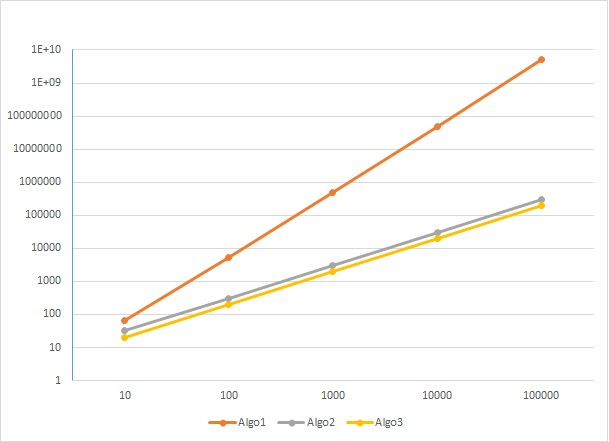
\includegraphics[width=10cm]{img_graph}
\end{center}

La représentation graphique des résultats montre clairement la différence de croissance du nombre d'opérations de chaque algorithmes. 

Puisque nous utilisons une échelle logarithmique, l'algorithme 2 et 3 ont une pente identique. L'écart entre les deux droites est directement lié au facteur s'appliquant à la variable $n$. Le terme constant de l'algorithme 2 est totalement négligeable dès que $n$ augmente.

La pente de la droite de l'algorithme 1 est plus importante, illustrant la croissance plus rapide du nombre d'opérations lorsque le degré du polynôme augmente.

\end{document}